% Options for packages loaded elsewhere
\PassOptionsToPackage{unicode}{hyperref}
\PassOptionsToPackage{hyphens}{url}
\documentclass[
  ignorenonframetext,
]{beamer}
\newif\ifbibliography
\usepackage{pgfpages}
\setbeamertemplate{caption}[numbered]
\setbeamertemplate{caption label separator}{: }
\setbeamercolor{caption name}{fg=normal text.fg}
\beamertemplatenavigationsymbolsempty
% remove section numbering
\setbeamertemplate{part page}{
  \centering
  \begin{beamercolorbox}[sep=16pt,center]{part title}
    \usebeamerfont{part title}\insertpart\par
  \end{beamercolorbox}
}
\setbeamertemplate{section page}{
  \centering
  \begin{beamercolorbox}[sep=12pt,center]{section title}
    \usebeamerfont{section title}\insertsection\par
  \end{beamercolorbox}
}
\setbeamertemplate{subsection page}{
  \centering
  \begin{beamercolorbox}[sep=8pt,center]{subsection title}
    \usebeamerfont{subsection title}\insertsubsection\par
  \end{beamercolorbox}
}
% Prevent slide breaks in the middle of a paragraph
\widowpenalties 1 10000
\raggedbottom
\AtBeginPart{
  \frame{\partpage}
}
\AtBeginSection{
  \ifbibliography
  \else
    \frame{\sectionpage}
  \fi
}
\AtBeginSubsection{
  \frame{\subsectionpage}
}
\usepackage{iftex}
\ifPDFTeX
  \usepackage[T1]{fontenc}
  \usepackage[utf8]{inputenc}
  \usepackage{textcomp} % provide euro and other symbols
\else % if luatex or xetex
  \usepackage{unicode-math} % this also loads fontspec
  \defaultfontfeatures{Scale=MatchLowercase}
  \defaultfontfeatures[\rmfamily]{Ligatures=TeX,Scale=1}
\fi
\usepackage{lmodern}
\ifPDFTeX\else
  % xetex/luatex font selection
\fi
% Use upquote if available, for straight quotes in verbatim environments
\IfFileExists{upquote.sty}{\usepackage{upquote}}{}
\IfFileExists{microtype.sty}{% use microtype if available
  \usepackage[]{microtype}
  \UseMicrotypeSet[protrusion]{basicmath} % disable protrusion for tt fonts
}{}
\makeatletter
\@ifundefined{KOMAClassName}{% if non-KOMA class
  \IfFileExists{parskip.sty}{%
    \usepackage{parskip}
  }{% else
    \setlength{\parindent}{0pt}
    \setlength{\parskip}{6pt plus 2pt minus 1pt}}
}{% if KOMA class
  \KOMAoptions{parskip=half}}
\makeatother
\usepackage{longtable,booktabs,array}
\newcounter{none} % for unnumbered tables
\usepackage{calc} % for calculating minipage widths
\usepackage{caption}
% Make caption package work with longtable
\makeatletter
\def\fnum@table{\tablename~\thetable}
\makeatother
\usepackage{graphicx}
\makeatletter
\newsavebox\pandoc@box
\newcommand*\pandocbounded[1]{% scales image to fit in text height/width
  \sbox\pandoc@box{#1}%
  \Gscale@div\@tempa{\textheight}{\dimexpr\ht\pandoc@box+\dp\pandoc@box\relax}%
  \Gscale@div\@tempb{\linewidth}{\wd\pandoc@box}%
  \ifdim\@tempb\p@<\@tempa\p@\let\@tempa\@tempb\fi% select the smaller of both
  \ifdim\@tempa\p@<\p@\scalebox{\@tempa}{\usebox\pandoc@box}%
  \else\usebox{\pandoc@box}%
  \fi%
}
% Set default figure placement to htbp
\def\fps@figure{htbp}
\makeatother
\setlength{\emergencystretch}{3em} % prevent overfull lines
\providecommand{\tightlist}{%
  \setlength{\itemsep}{0pt}\setlength{\parskip}{0pt}}
% Slide layout defaults for warning-clean scientific decks.
\usepackage{etoolbox}
\IfFileExists{xurl.sty}{\usepackage{xurl}}{}
\IfFileExists{seqsplit.sty}{\usepackage{seqsplit}}{\newcommand{\seqsplit}[1]{#1}}
\protected\def\breakseq#1{\seqsplit{#1}}
\protected\def\breaktt#1{\begingroup\ttfamily\seqsplit{#1}\endgroup}
\setlength{\emergencystretch}{6em}
\tolerance=5000
\hbadness=10000
\hfuzz=1pt
\setlength{\tabcolsep}{2pt}
\AtBeginEnvironment{longtable}{\tiny\renewcommand{\arraystretch}{0.86}\setlength{\tabcolsep}{1pt}}
\AtBeginEnvironment{tabular}{\tiny\renewcommand{\arraystretch}{0.86}\setlength{\tabcolsep}{1pt}}

% Natbib and cross-reference fallbacks — slides don't load natbib
% or cleveref, but combined-PDF manuscript prose may emit these
% commands. The fallback renders citations as a bracketed key list
% and cross-references as detokenized labels so slides don't fail on
% undefined control sequences or raw underscores. \providecommand is
% a no-op if packages load later.
\providecommand{\citep}[1]{[#1]}
\providecommand{\citet}[1]{#1}
\providecommand{\citealp}[1]{#1}
\providecommand{\citeauthor}[1]{#1}
\providecommand{\citeyear}[1]{#1}
\providecommand{\cref}[1]{\texttt{\detokenize{#1}}}
\providecommand{\Cref}[1]{\texttt{\detokenize{#1}}}

\newtheorem{proposition}{Proposition}
\newtheorem{hypothesis}{Hypothesis}
\usepackage{bookmark}
\IfFileExists{xurl.sty}{\usepackage{xurl}}{} % add URL line breaks if available
\urlstyle{same}
% fallback for those not using the hyperref driver hyperxmp:
\makeatletter
\@ifundefined{xmpquote}{\newcommand{\xmpquote}[1]{#1}}{}
\makeatother
\hypersetup{
  hidelinks,
  pdfcreator={LaTeX via pandoc}}

\author{\texorpdfstring{}{}}
\date{}

\begin{document}

\section{Results: Field Overview}\label{results-field-overview}

\begin{frame}[allowframebreaks]{Results: Field Overview}
The de-duplicated corpus for \textbf{Modafinil} contains \(N = 2302\)
records spanning 2000--2026 (26 years). Publication volume grows at a
compound annual rate of 3.45\% (mean year-over-year growth 6.3\%,
doubling time 11.3 years), peaking in 2025 with 112 records that year.
The growth curve is the first-order signal that the literature is active
rather than dormant.

\pandocbounded{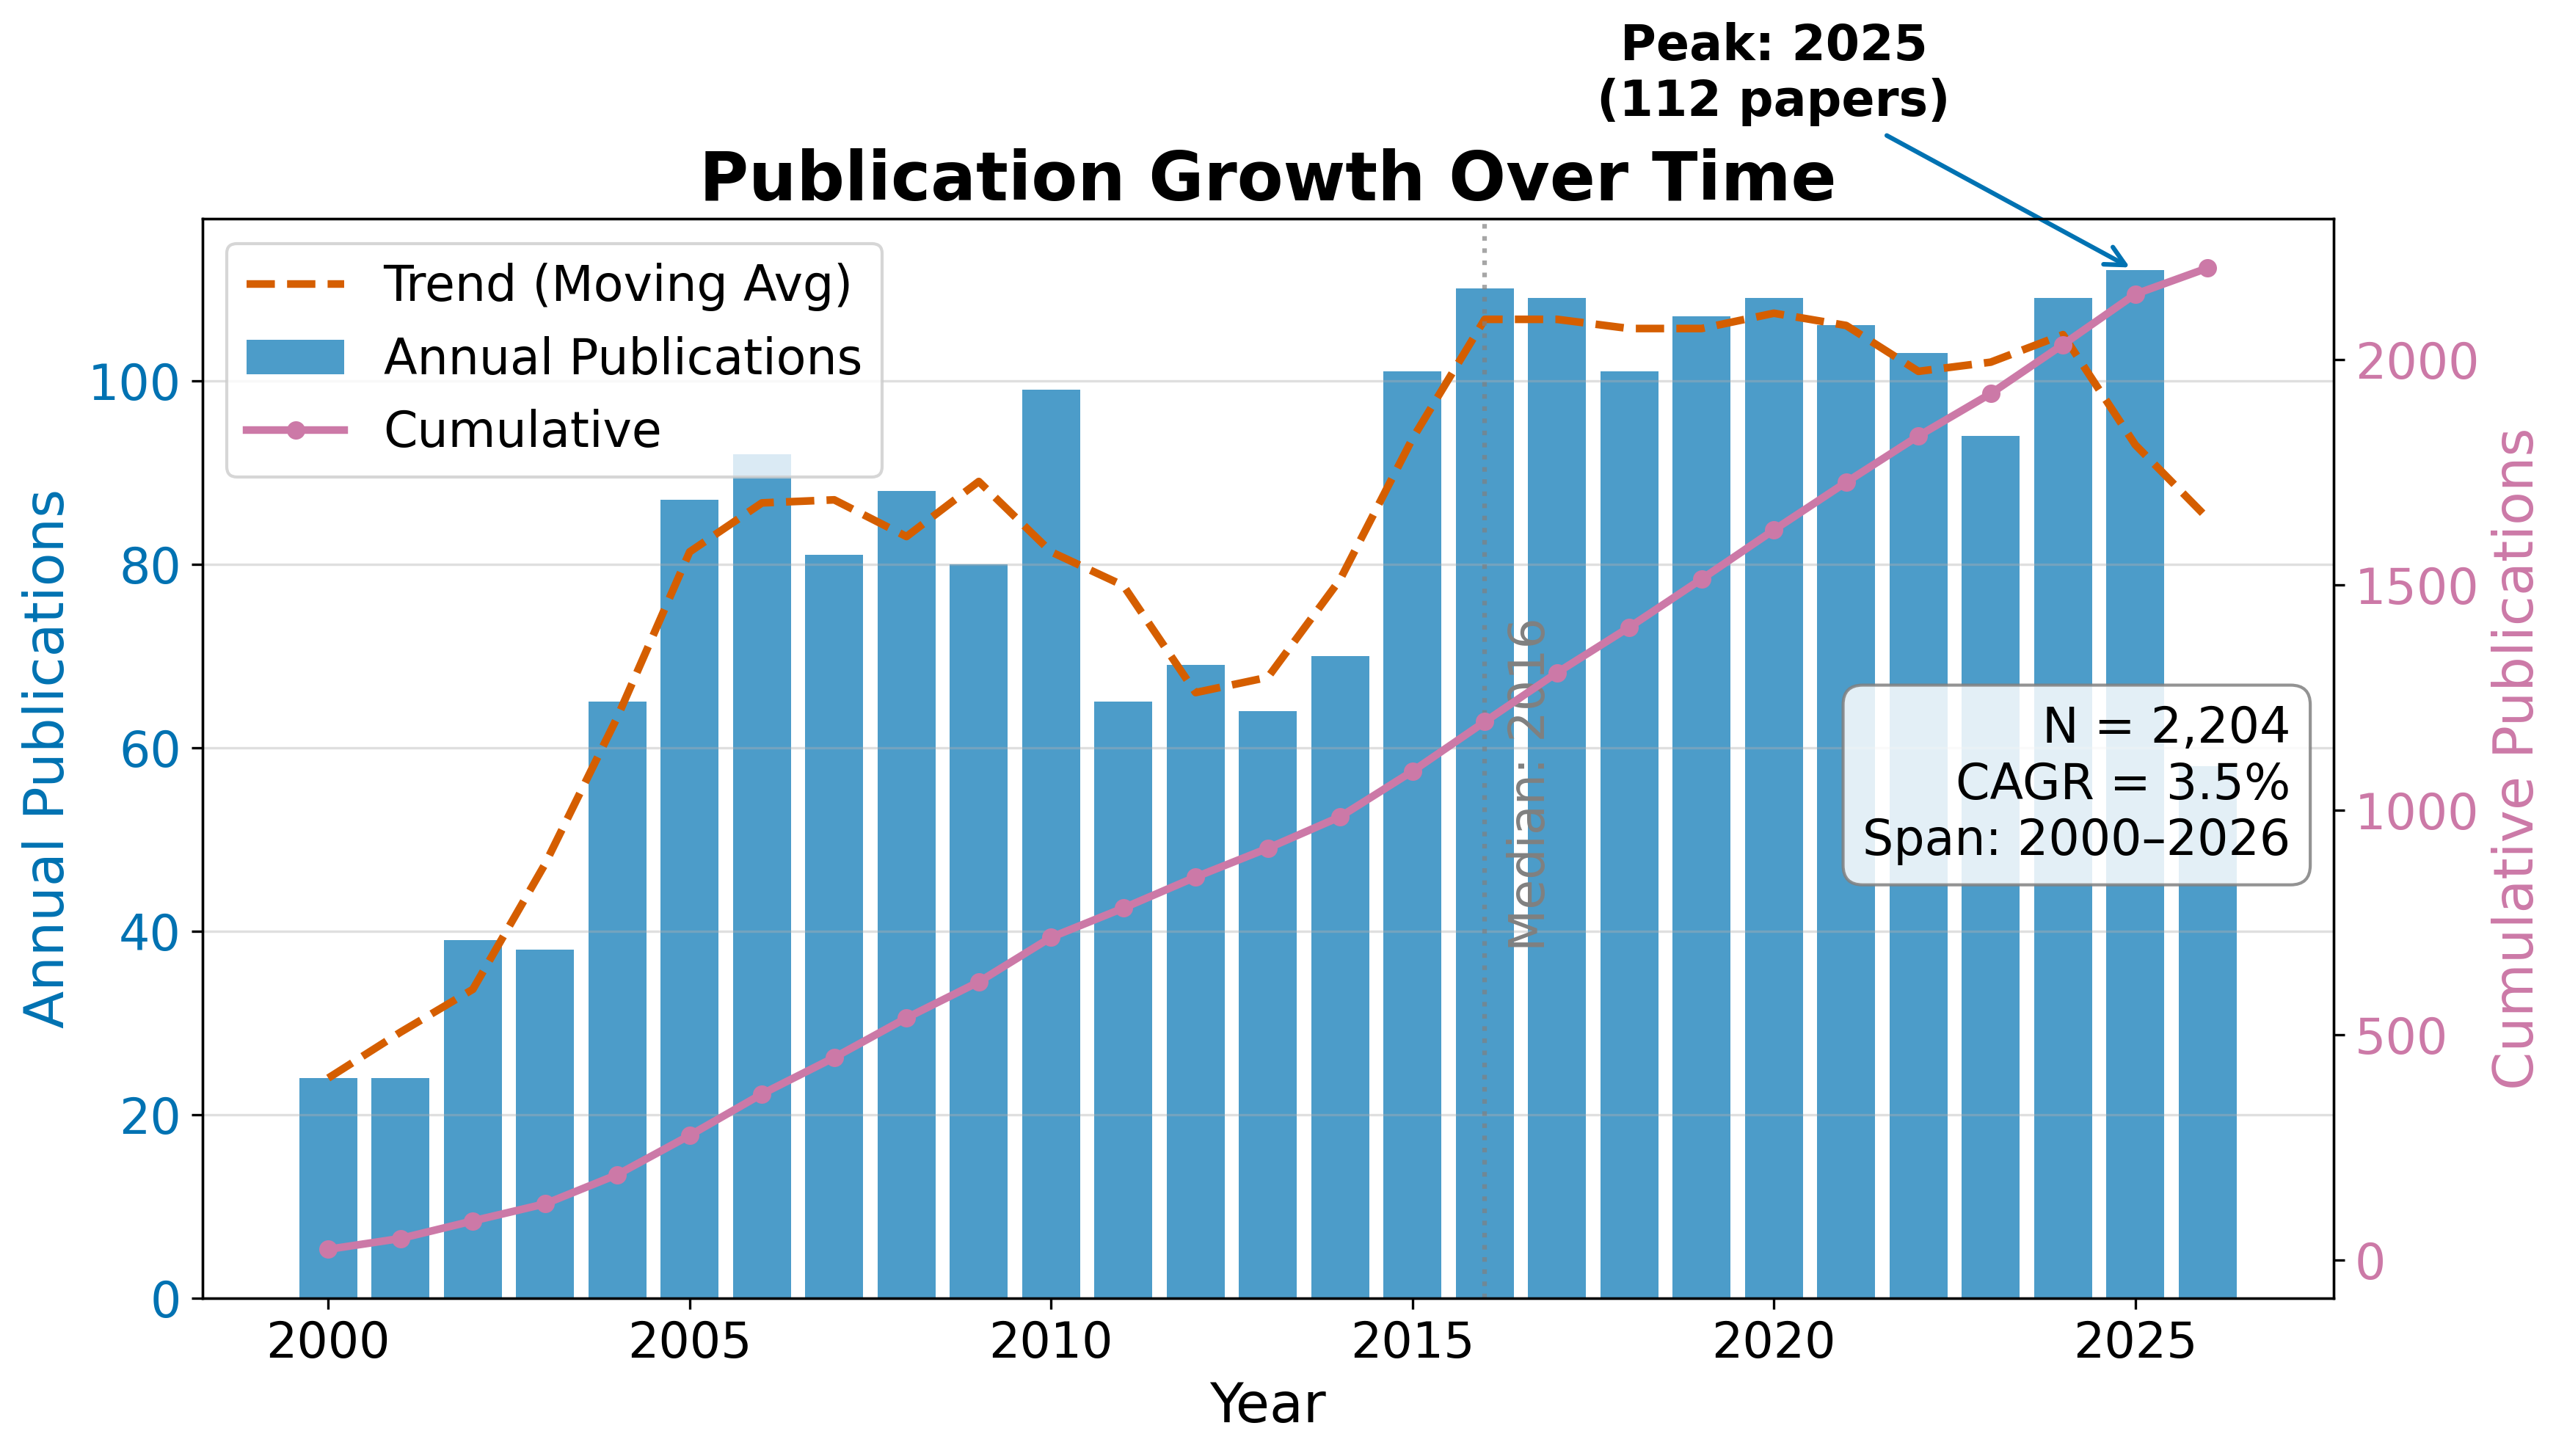
\includegraphics[keepaspectratio,alt={Publication growth curve for Modafinil. Annual publication counts (bars) and cumulative total (line) show sustained growth from 2000 through 2026, peaking in 2025.}]{../figures/growth_curve.png}}\{\{\#fig:growth\_curve\}\}
\end{frame}

\begin{frame}[allowframebreaks]{RQ1: Field Size and Growth}
\protect\phantomsection\label{rq1-field-size-and-growth}
The temporal analysis reveals a literature that has grown steadily over
26 years. The compound annual growth rate of 3.45\% means the corpus
roughly doubles every 11.3 years --- a pace that exceeds the general
biomedical literature growth rate of approximately 4\% per year. The
peak year 2025 with 112 publications likely reflects both genuine
research activity and the lag between publication and indexing in the
source databases.

\textbf{Table 1. Top publication years.}

{\def\LTcaptype{none} % do not increment counter
\begin{longtable}[]{@{}ll@{}}
\toprule\noalign{}
Year & Publications \\
\midrule\noalign{}
\endhead
2015 & 101 \\
2016 & 110 \\
2017 & 109 \\
2018 & 101 \\
2019 & 107 \\
2020 & 109 \\
2021 & 106 \\
2022 & 103 \\
2024 & 109 \\
2025 & 112 \\
\bottomrule\noalign{}
\end{longtable}
}
\end{frame}

\begin{frame}[allowframebreaks]{RQ2: Subfield Composition}
\protect\phantomsection\label{rq2-subfield-composition}
Records distribute across the 6 configured subfields as shown in Table
2, with \textbf{Clinical Sleep} the largest bucket at 64.3\% of the
classified corpus. The dominance of Clinical Sleep reflects the clinical
primacy of modafinil as a wakefulness-promoting agent: the largest body
of literature addresses its use in narcolepsy, shift-work disorder, and
obstructive sleep apnea.

\textbf{Table 2. Subfield distribution.}

{\def\LTcaptype{none} % do not increment counter
\begin{longtable}[]{@{}lll@{}}
\toprule\noalign{}
Subfield & Papers & Share \\
\midrule\noalign{}
\endhead
Clinical Sleep & 1417 & 64.3\% \\
Cognition & 233 & 10.6\% \\
Pharmacology & 74 & 3.4\% \\
Psychiatry & 357 & 16.2\% \\
Safety & 82 & 3.7\% \\
Neuroscience & 41 & 1.9\% \\
\bottomrule\noalign{}
\end{longtable}
}

\pandocbounded{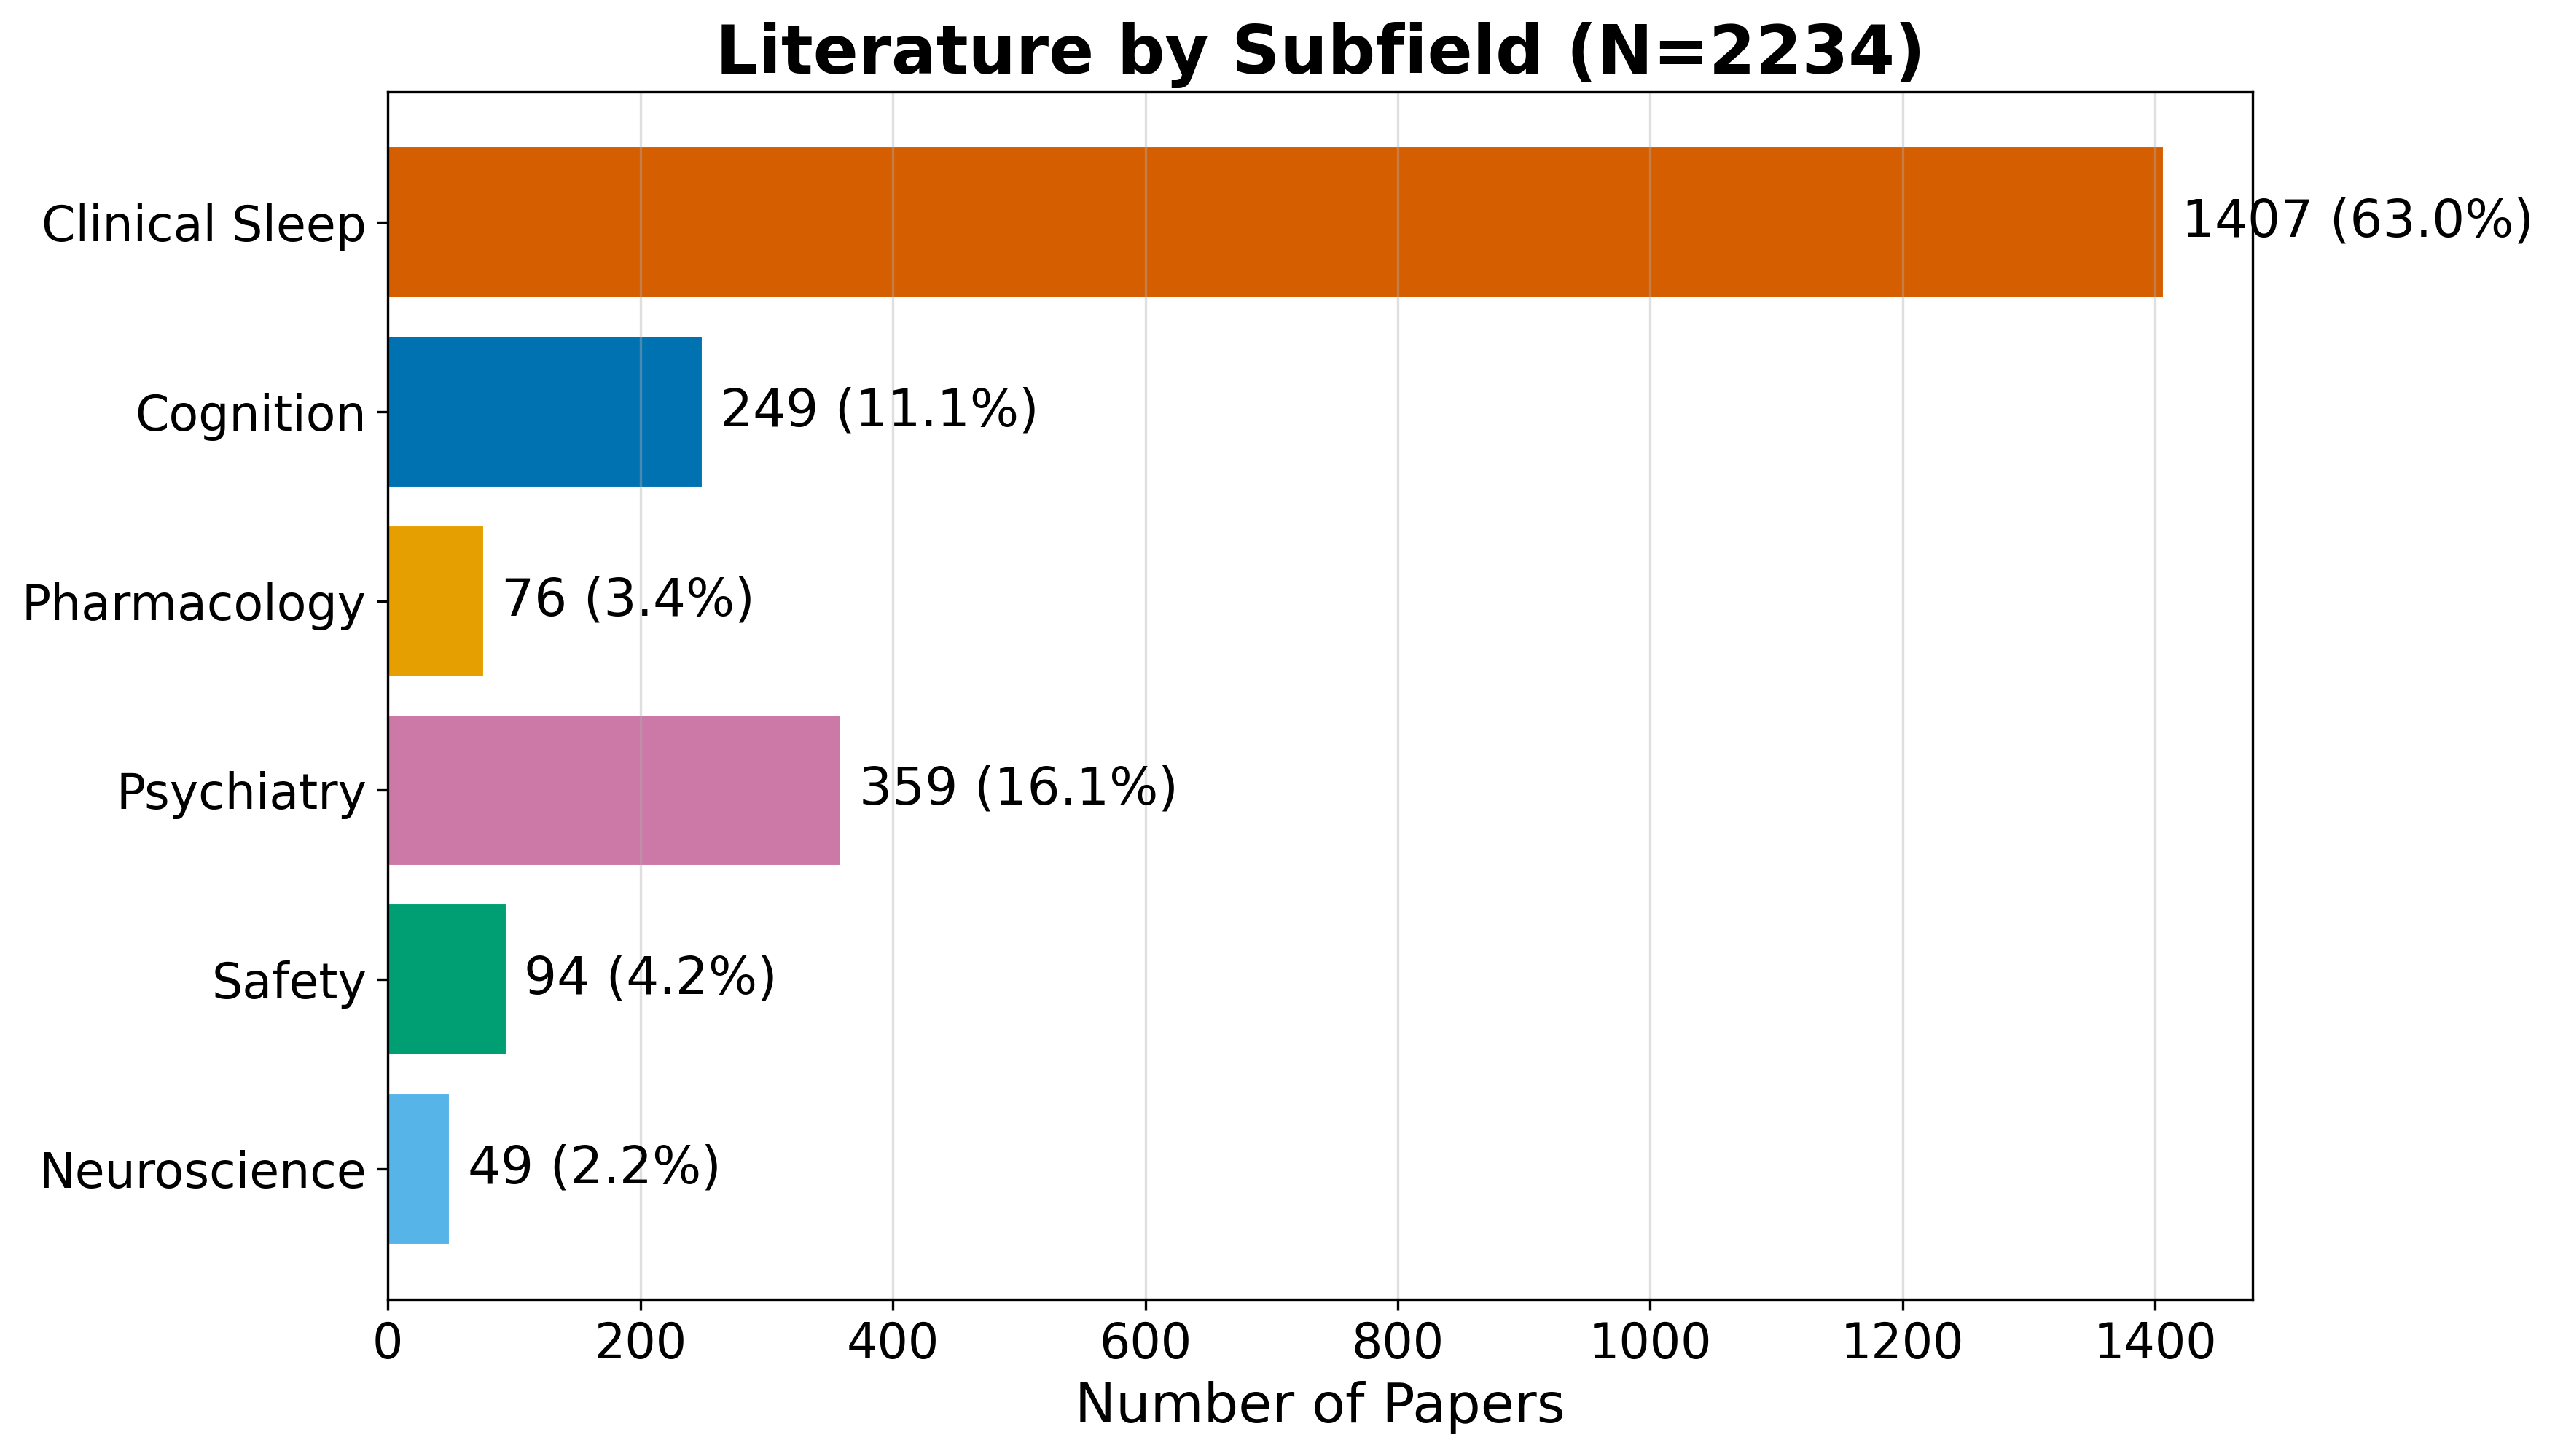
\includegraphics[keepaspectratio,alt={Field summary dashboard for Modafinil. The dashboard combines corpus size, temporal range, subfield distribution, and key bibliometric indicators in a single overview panel.}]{../figures/field_summary.png}}\{\{\#fig:field\_summary\}\}

\pandocbounded{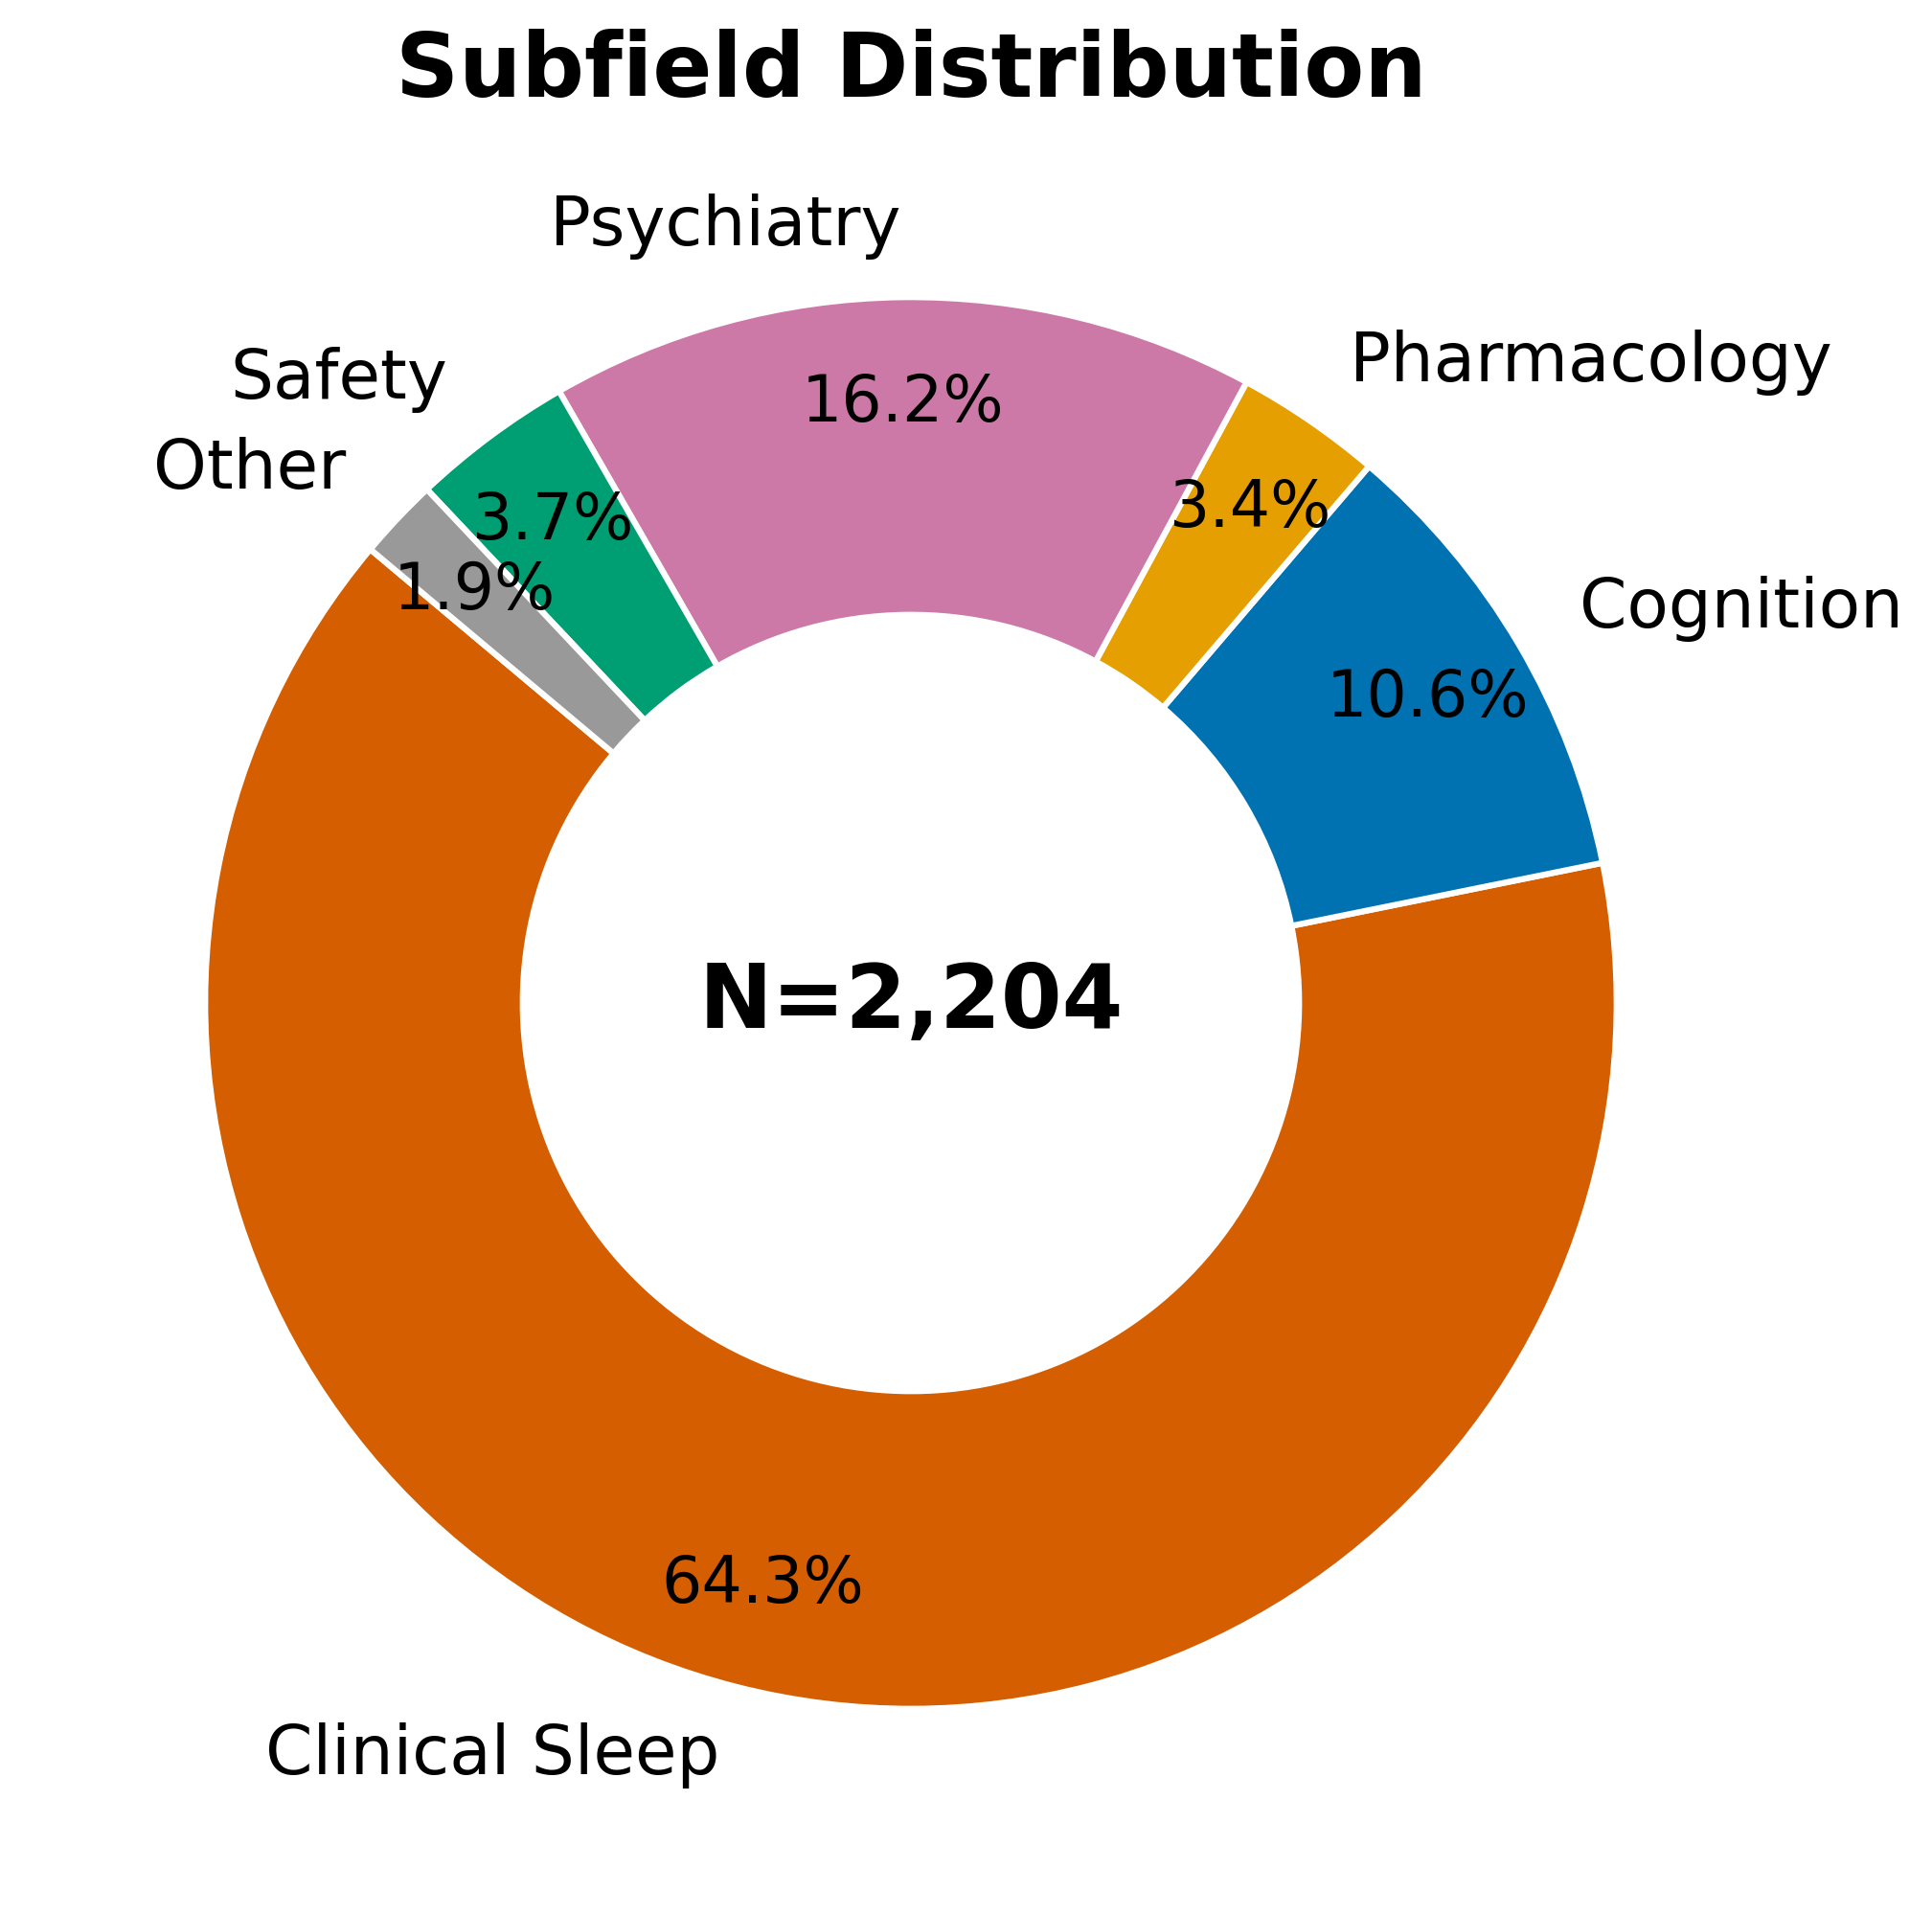
\includegraphics[keepaspectratio,alt={Subfield distribution for Modafinil. The 6-bucket taxonomy shows the relative weight of each configured sub-area, with Clinical Sleep dominant at 64.3\%.}]{../figures/subfield_distribution.png}}\{\{\#fig:subfield\_distribution\}\}

\pandocbounded{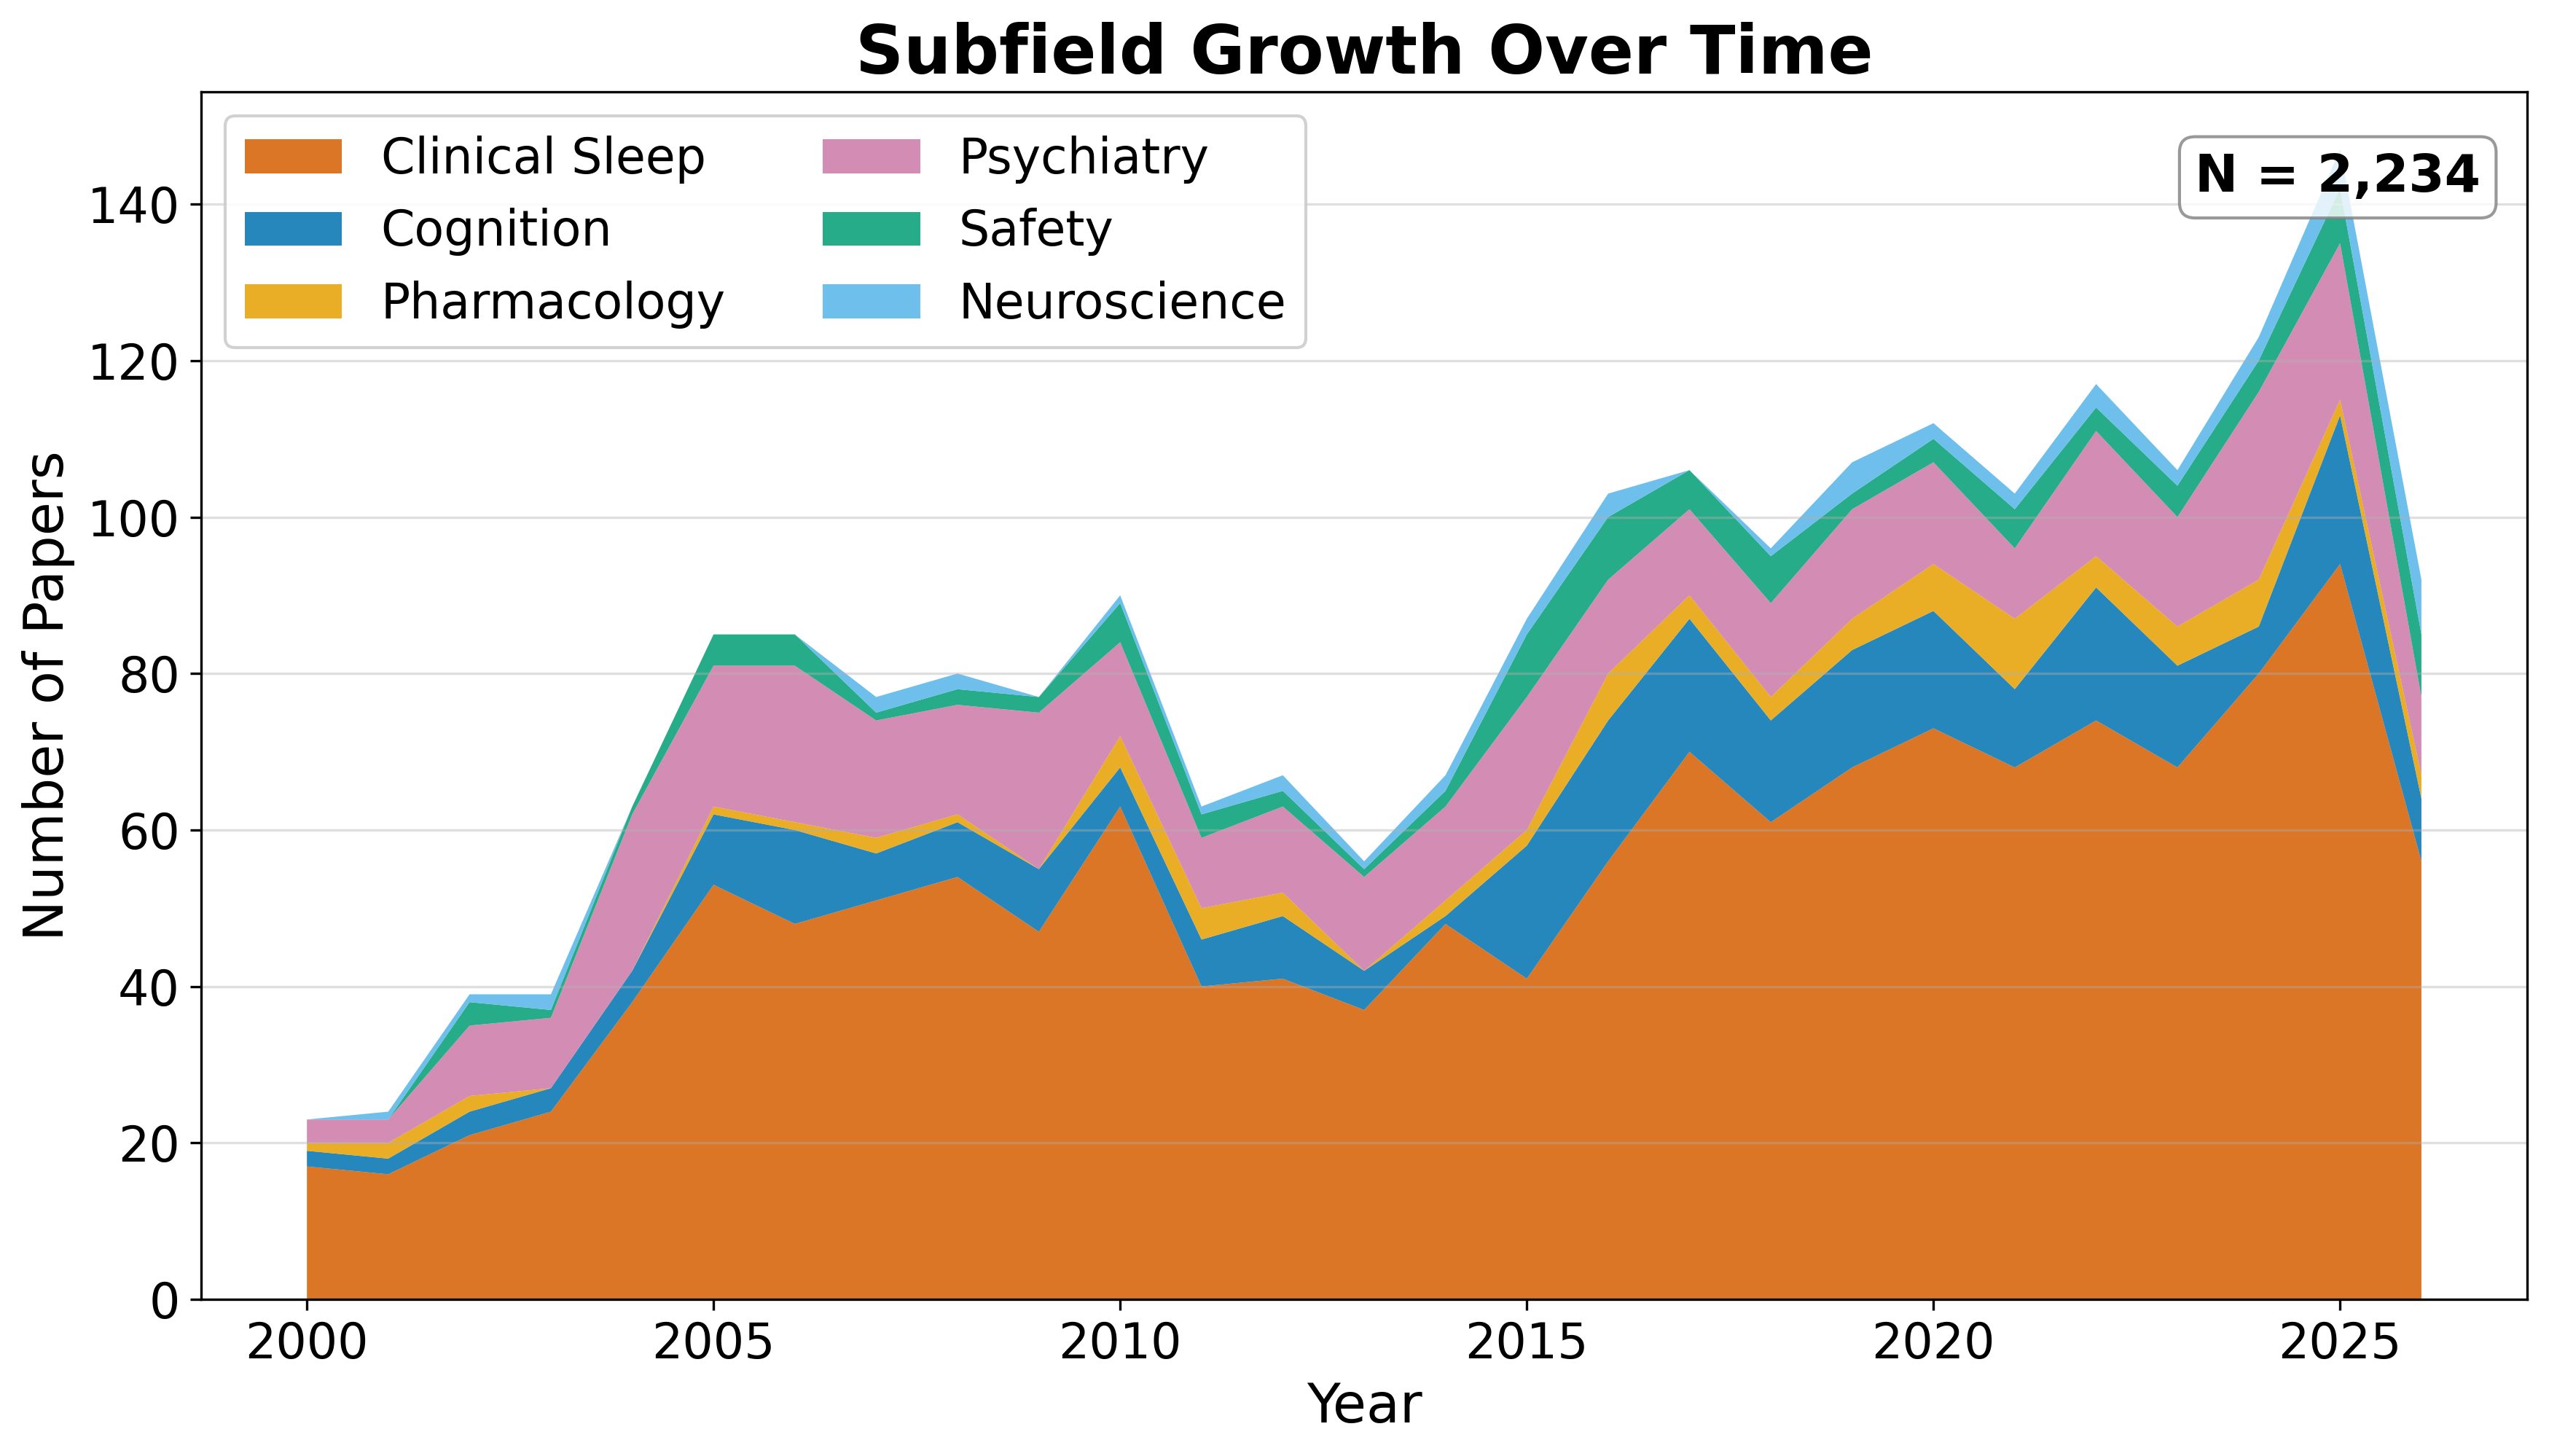
\includegraphics[keepaspectratio,alt={Subfield timeline for Modafinil. Stacked annual publication counts by subfield show how each sub-area has evolved over time, revealing emerging and declining research threads.}]{../figures/subfield_timeline.png}}\{\{\#fig:subfield\_timeline\}\}
\end{frame}

\begin{frame}[allowframebreaks]{Identifier and Full-Text Coverage}
\protect\phantomsection\label{identifier-and-full-text-coverage}
The corpus has strong identifier coverage: 2248 of 2302 records (98.0\%)
carry DOIs, enabling robust cross-engine de-duplication. OpenAlex IDs
are present for 932 records. Abstract coverage stands at 55.5\% (1277
records), which limits the text analytics to that subset. Open-access
status is confirmed for 14.4\% of records, and 40.9\% have a direct PDF
link.
\end{frame}

\begin{frame}[allowframebreaks]{Descriptive Bibliometrics}
\protect\phantomsection\label{descriptive-bibliometrics}
The corpus spans 7259 unique authors across 2302 papers, yielding a mean
of 1.34 papers per author. Citation counts range from zero to 1333 (mean
30.9, median 0.0), with a total of 68,151 citations across the corpus.
The Gini coefficient of citation concentration is 0.812, indicating a
highly skewed distribution characteristic of scientific literature.

\textbf{Table 3. Citation count distribution.}

{\def\LTcaptype{none} % do not increment counter
\begin{longtable}[]{@{}ll@{}}
\toprule\noalign{}
Citations & Papers \\
\midrule\noalign{}
\endhead
0 & 1184 \\
1-9 & 195 \\
10-49 & 421 \\
50-99 & 214 \\
100-499 & 179 \\
500+ & 11 \\
\bottomrule\noalign{}
\end{longtable}
}

\pandocbounded{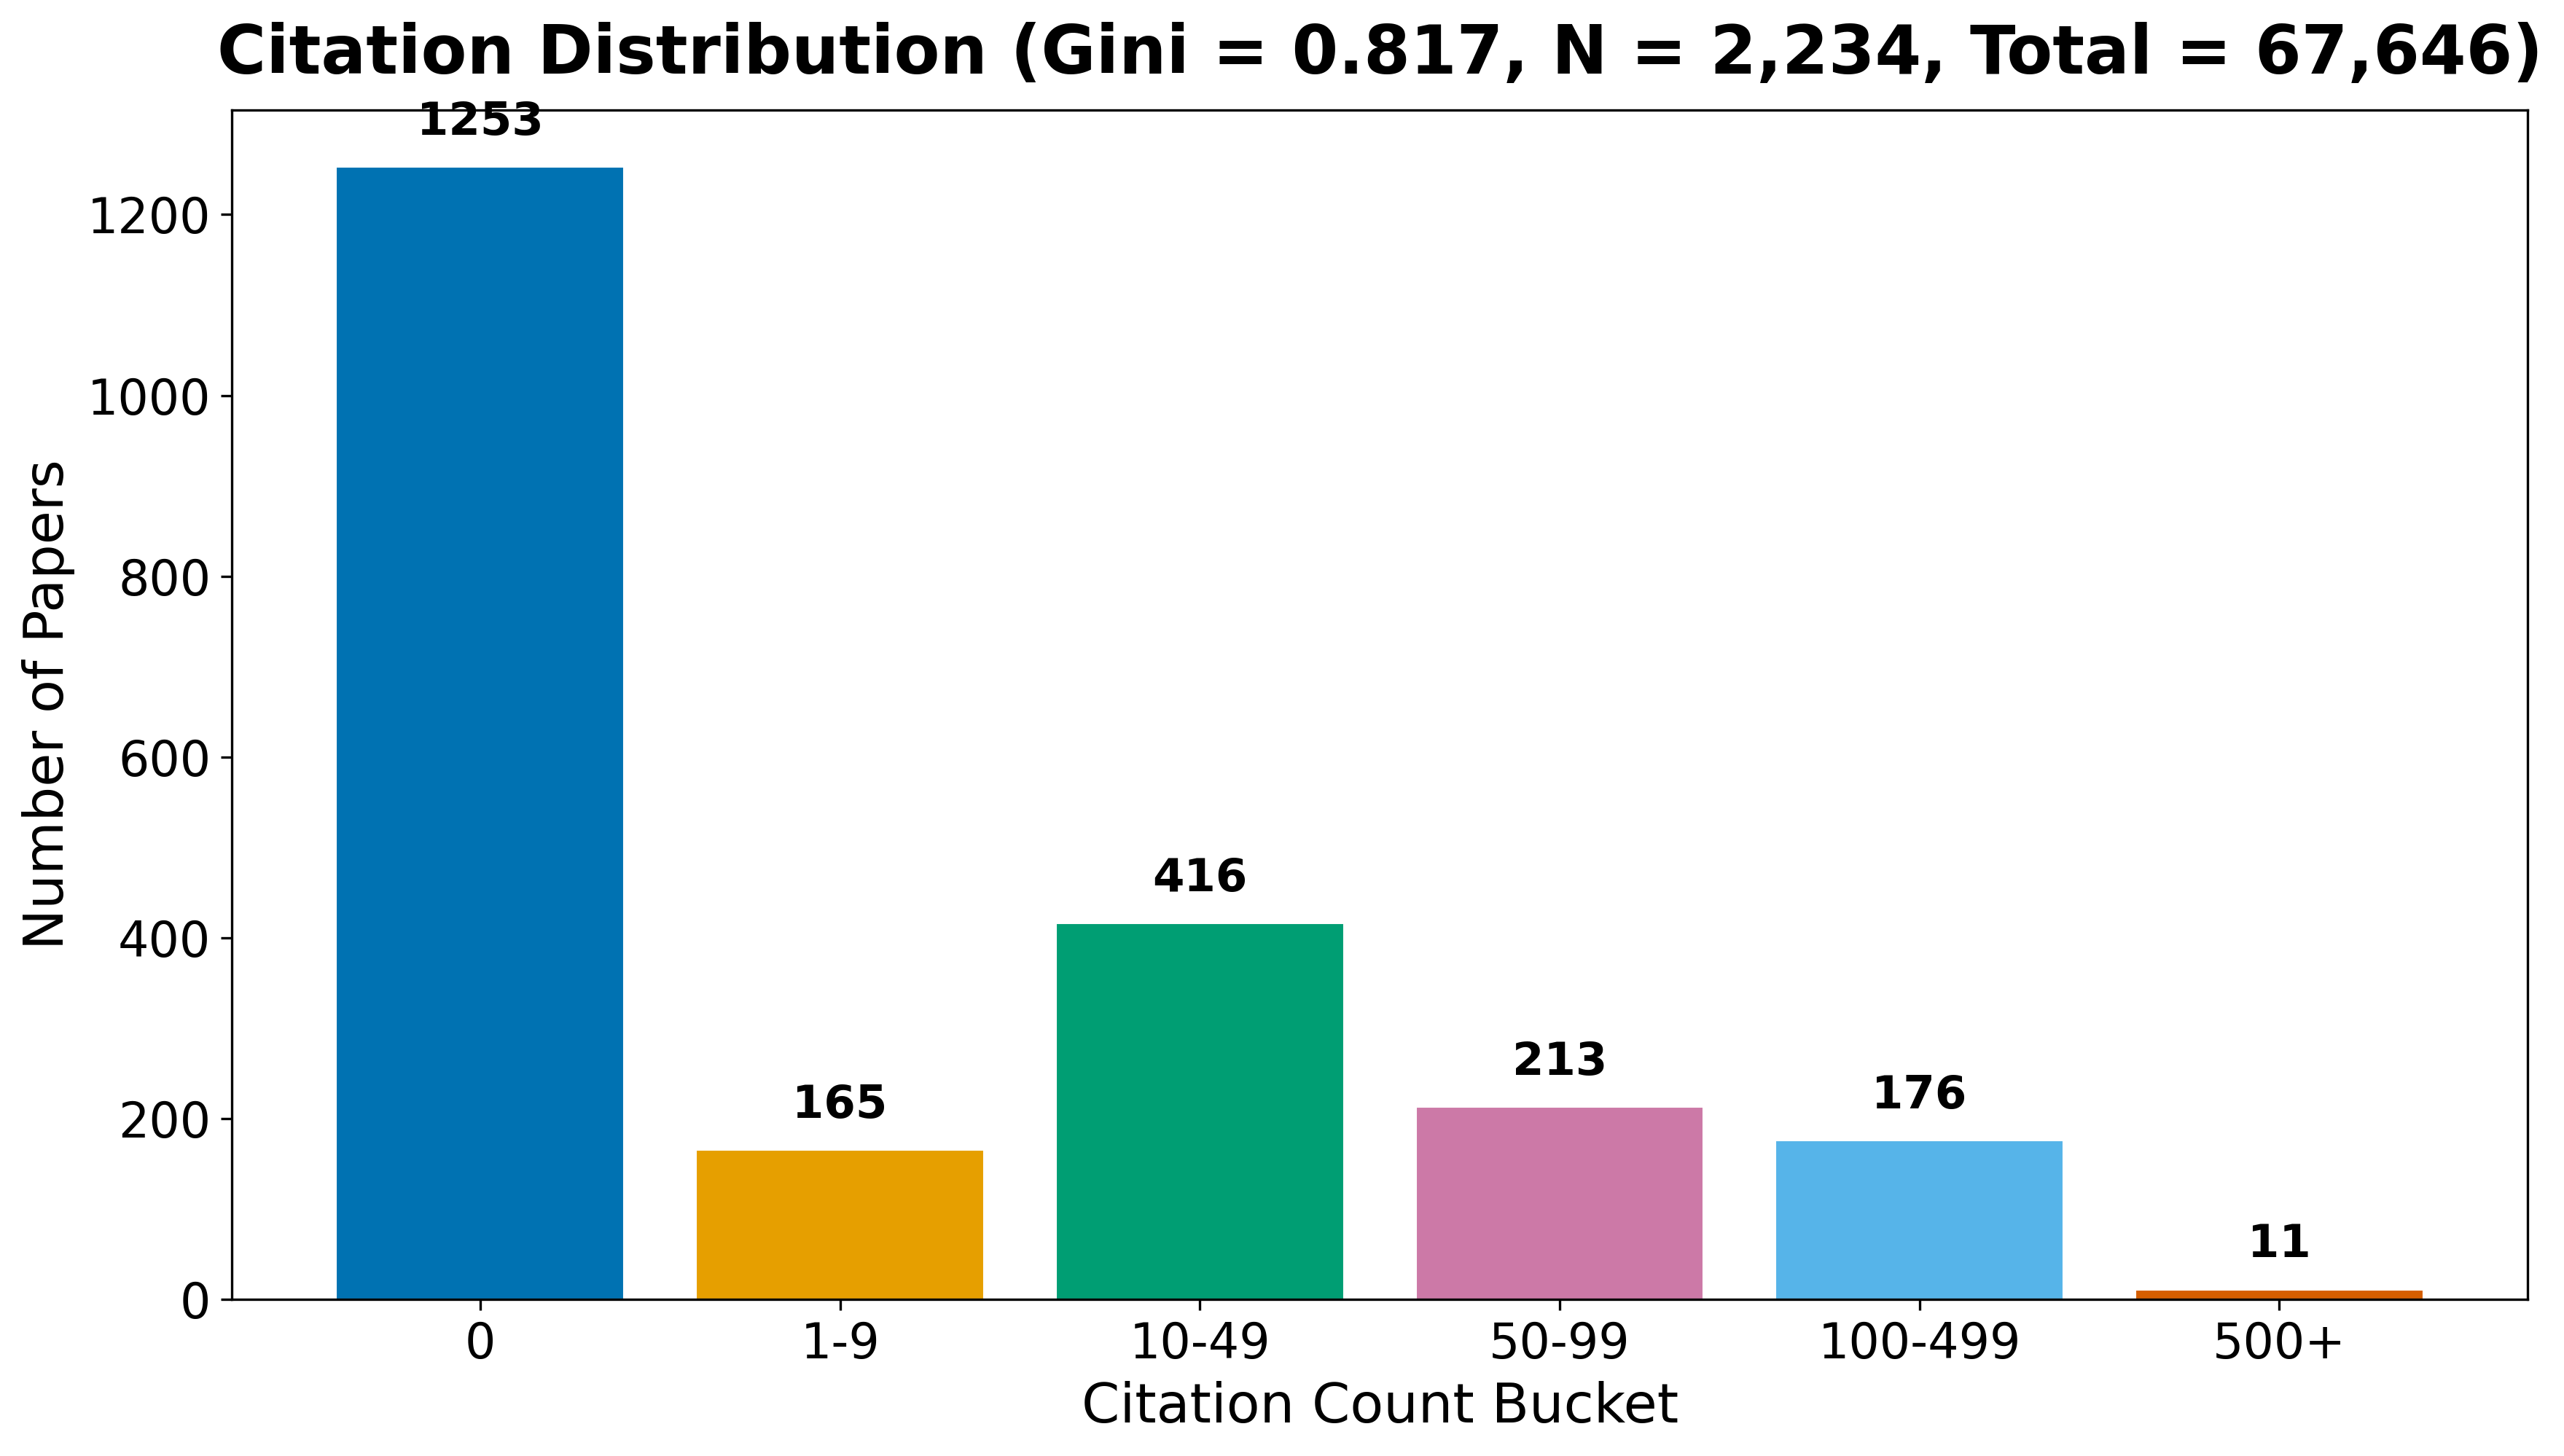
\includegraphics[keepaspectratio,alt={Citation distribution for Modafinil. The histogram shows the number of papers in each citation-count bucket, with the Gini coefficient annotated. The heavy-tailed distribution is characteristic of scientific citation networks.}]{../figures/citation_distribution.png}}\{\{\#fig:citation\_distribution\}\}

\textbf{Table 4. Top publication venues.}

{\def\LTcaptype{none} % do not increment counter
\begin{longtable}[]{@{}ll@{}}
\toprule\noalign{}
Venue & Papers \\
\midrule\noalign{}
\endhead
Reactions Weekly & 142 \\
Psychopharmacology & 41 \\
SLEEP & 34 \\
Sleep Medicine & 33 \\
The Journal of Clinical Psychiatry & 31 \\
European Neuropsychopharmacology & 27 \\
Neuropharmacology & 26 \\
Inpharma Weekly & 25 \\
PubMed & 24 \\
American Journal of Psychiatry & 23 \\
\bottomrule\noalign{}
\end{longtable}
}

\pandocbounded{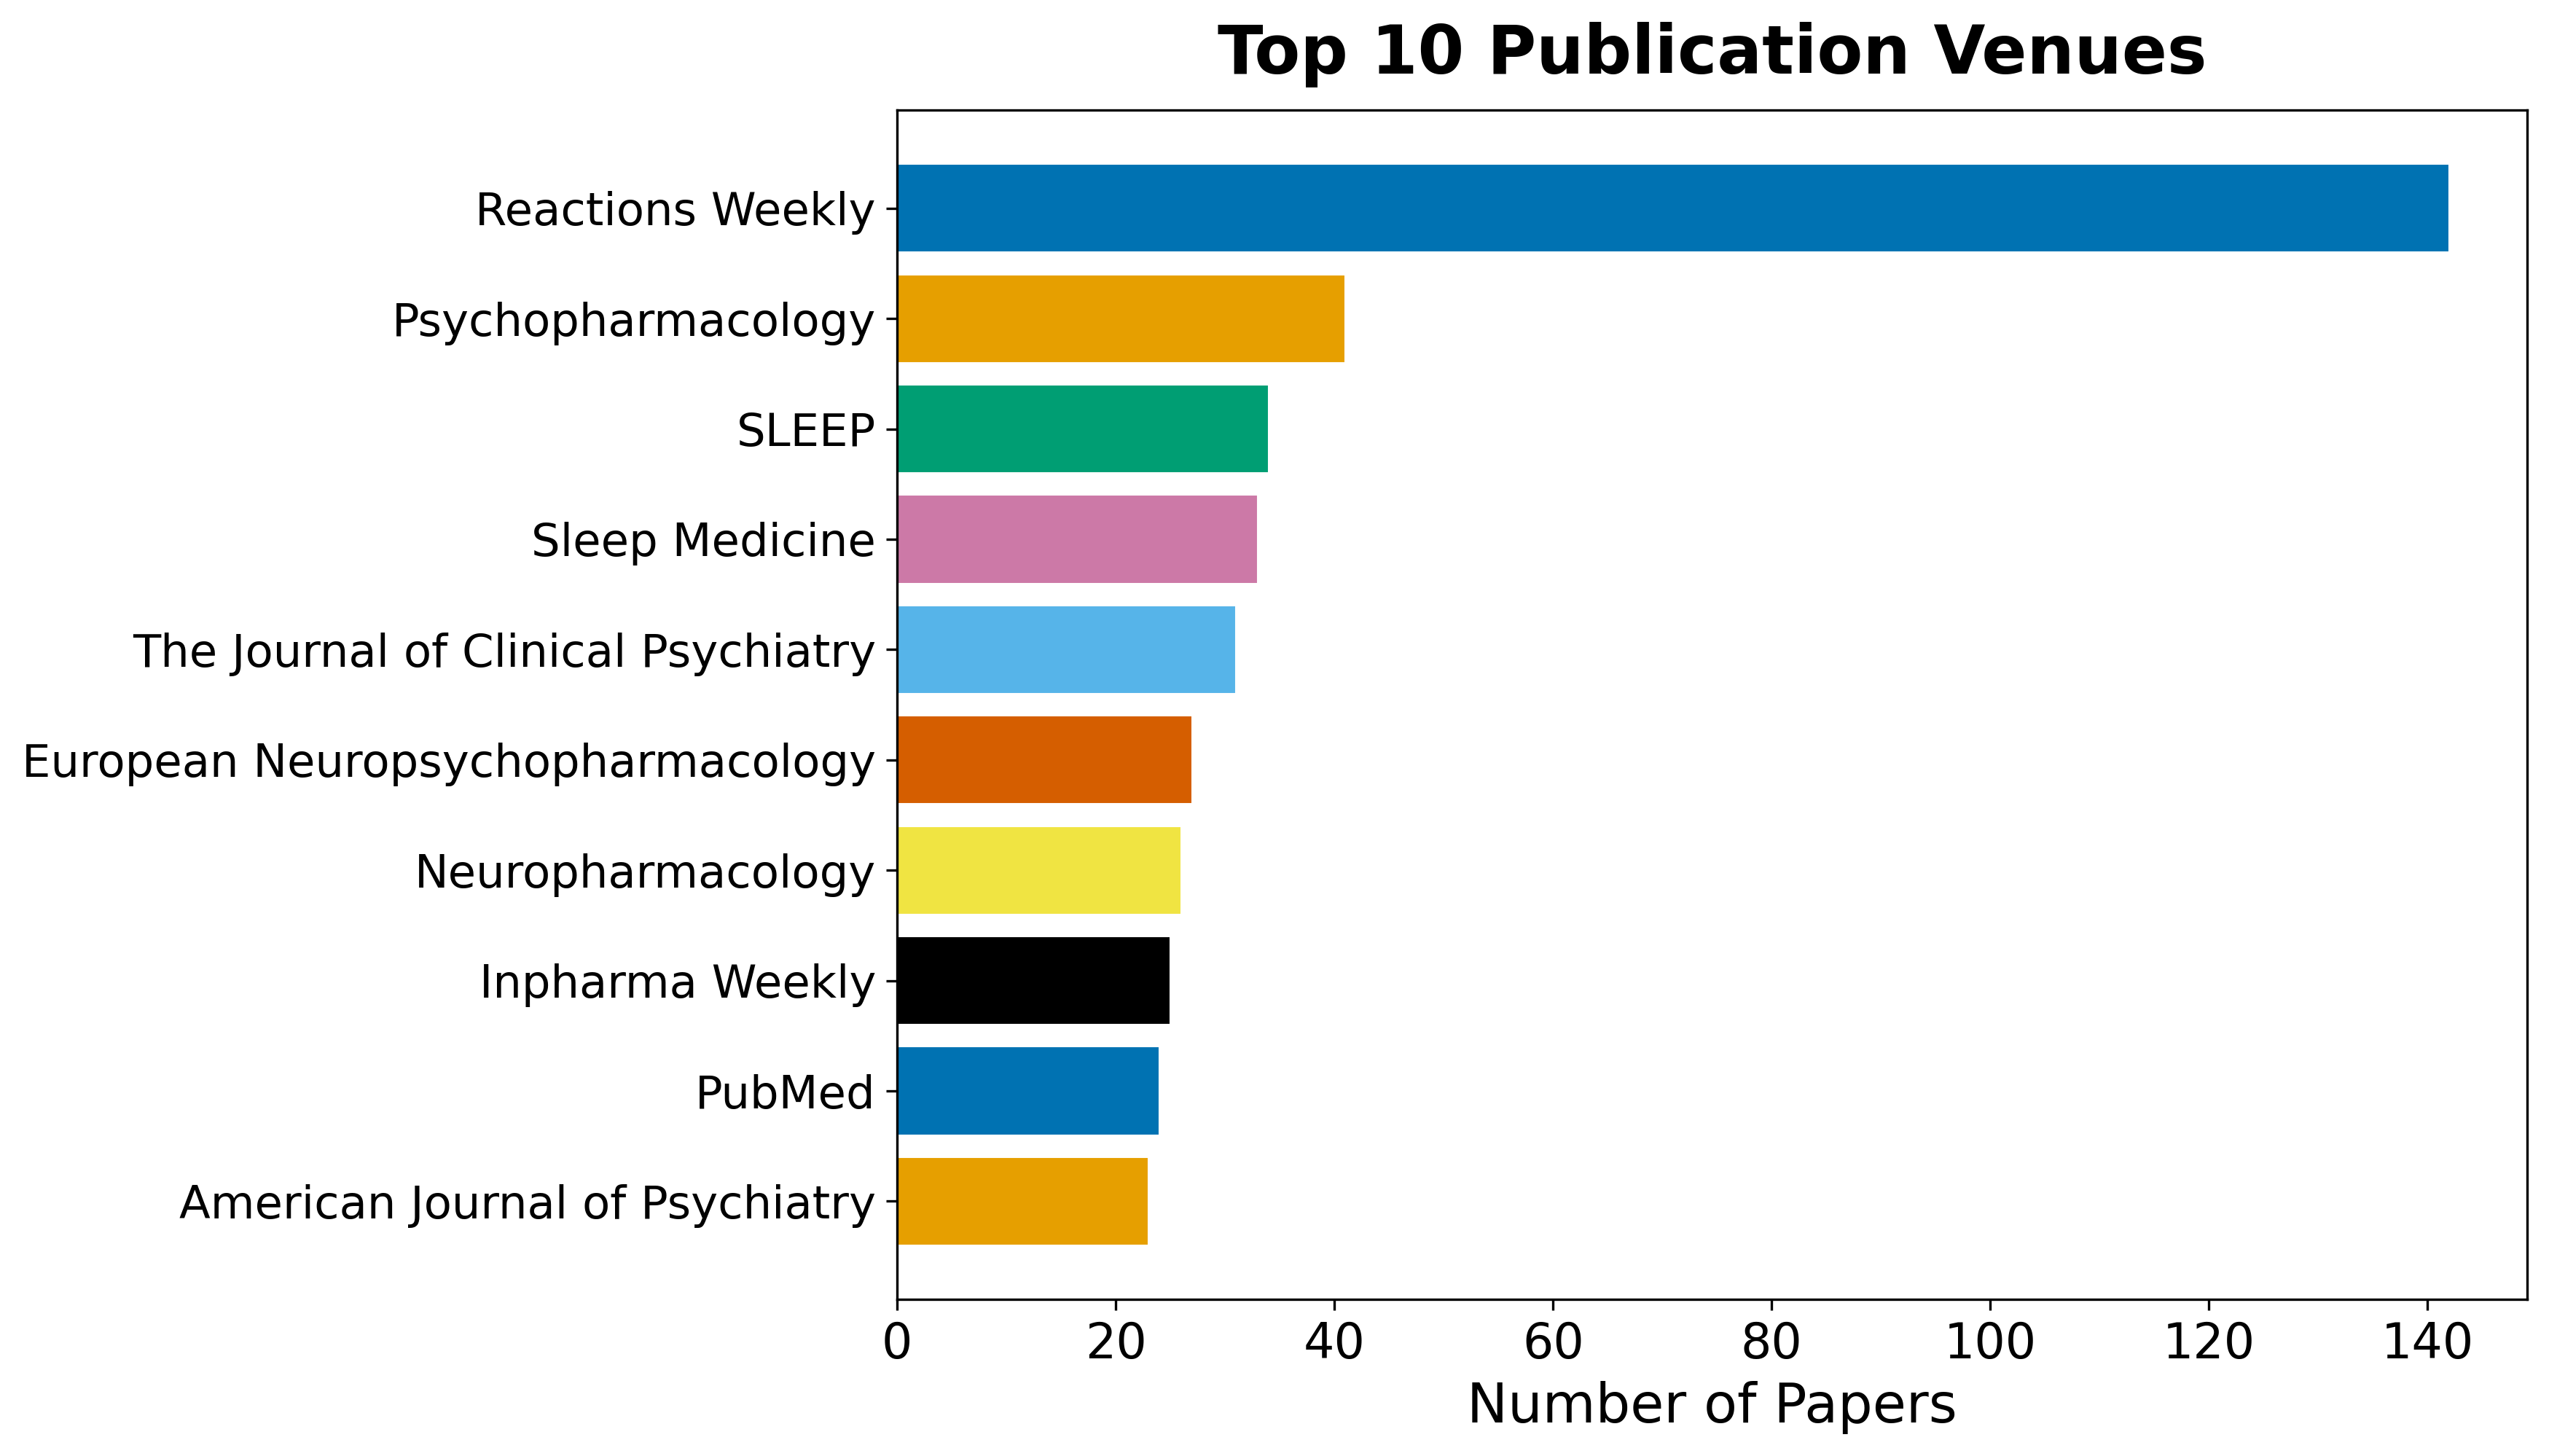
\includegraphics[keepaspectratio,alt={Top publication venues for Modafinil. The horizontal bar chart shows the 15 venues with the most papers in the corpus, revealing where the modafinil literature is published.}]{../figures/top_venues.png}}\{\{\#fig:top\_venues\}\}

\textbf{Table 5. Top authors by publication count.}

{\def\LTcaptype{none} % do not increment counter
\begin{longtable}[]{@{}lll@{}}
\toprule\noalign{}
Rank & Author & Papers \\
\midrule\noalign{}
\endhead
1 & \&NA; & 66 \\
2 & Ronghua Yang & 26 \\
3 & Yves Dauvilliers & 26 \\
4 & Amy Hauck Newman & 22 \\
5 & Barbara J. Sahakian & 20 \\
6 & Edward T. Hellriegel & 17 \\
7 & Gianluigi Tanda & 16 \\
8 & Philmore Robertson & 16 \\
9 & Sanjay Arora & 16 \\
10 & Gert Lubec & 15 \\
\bottomrule\noalign{}
\end{longtable}
}

\pandocbounded{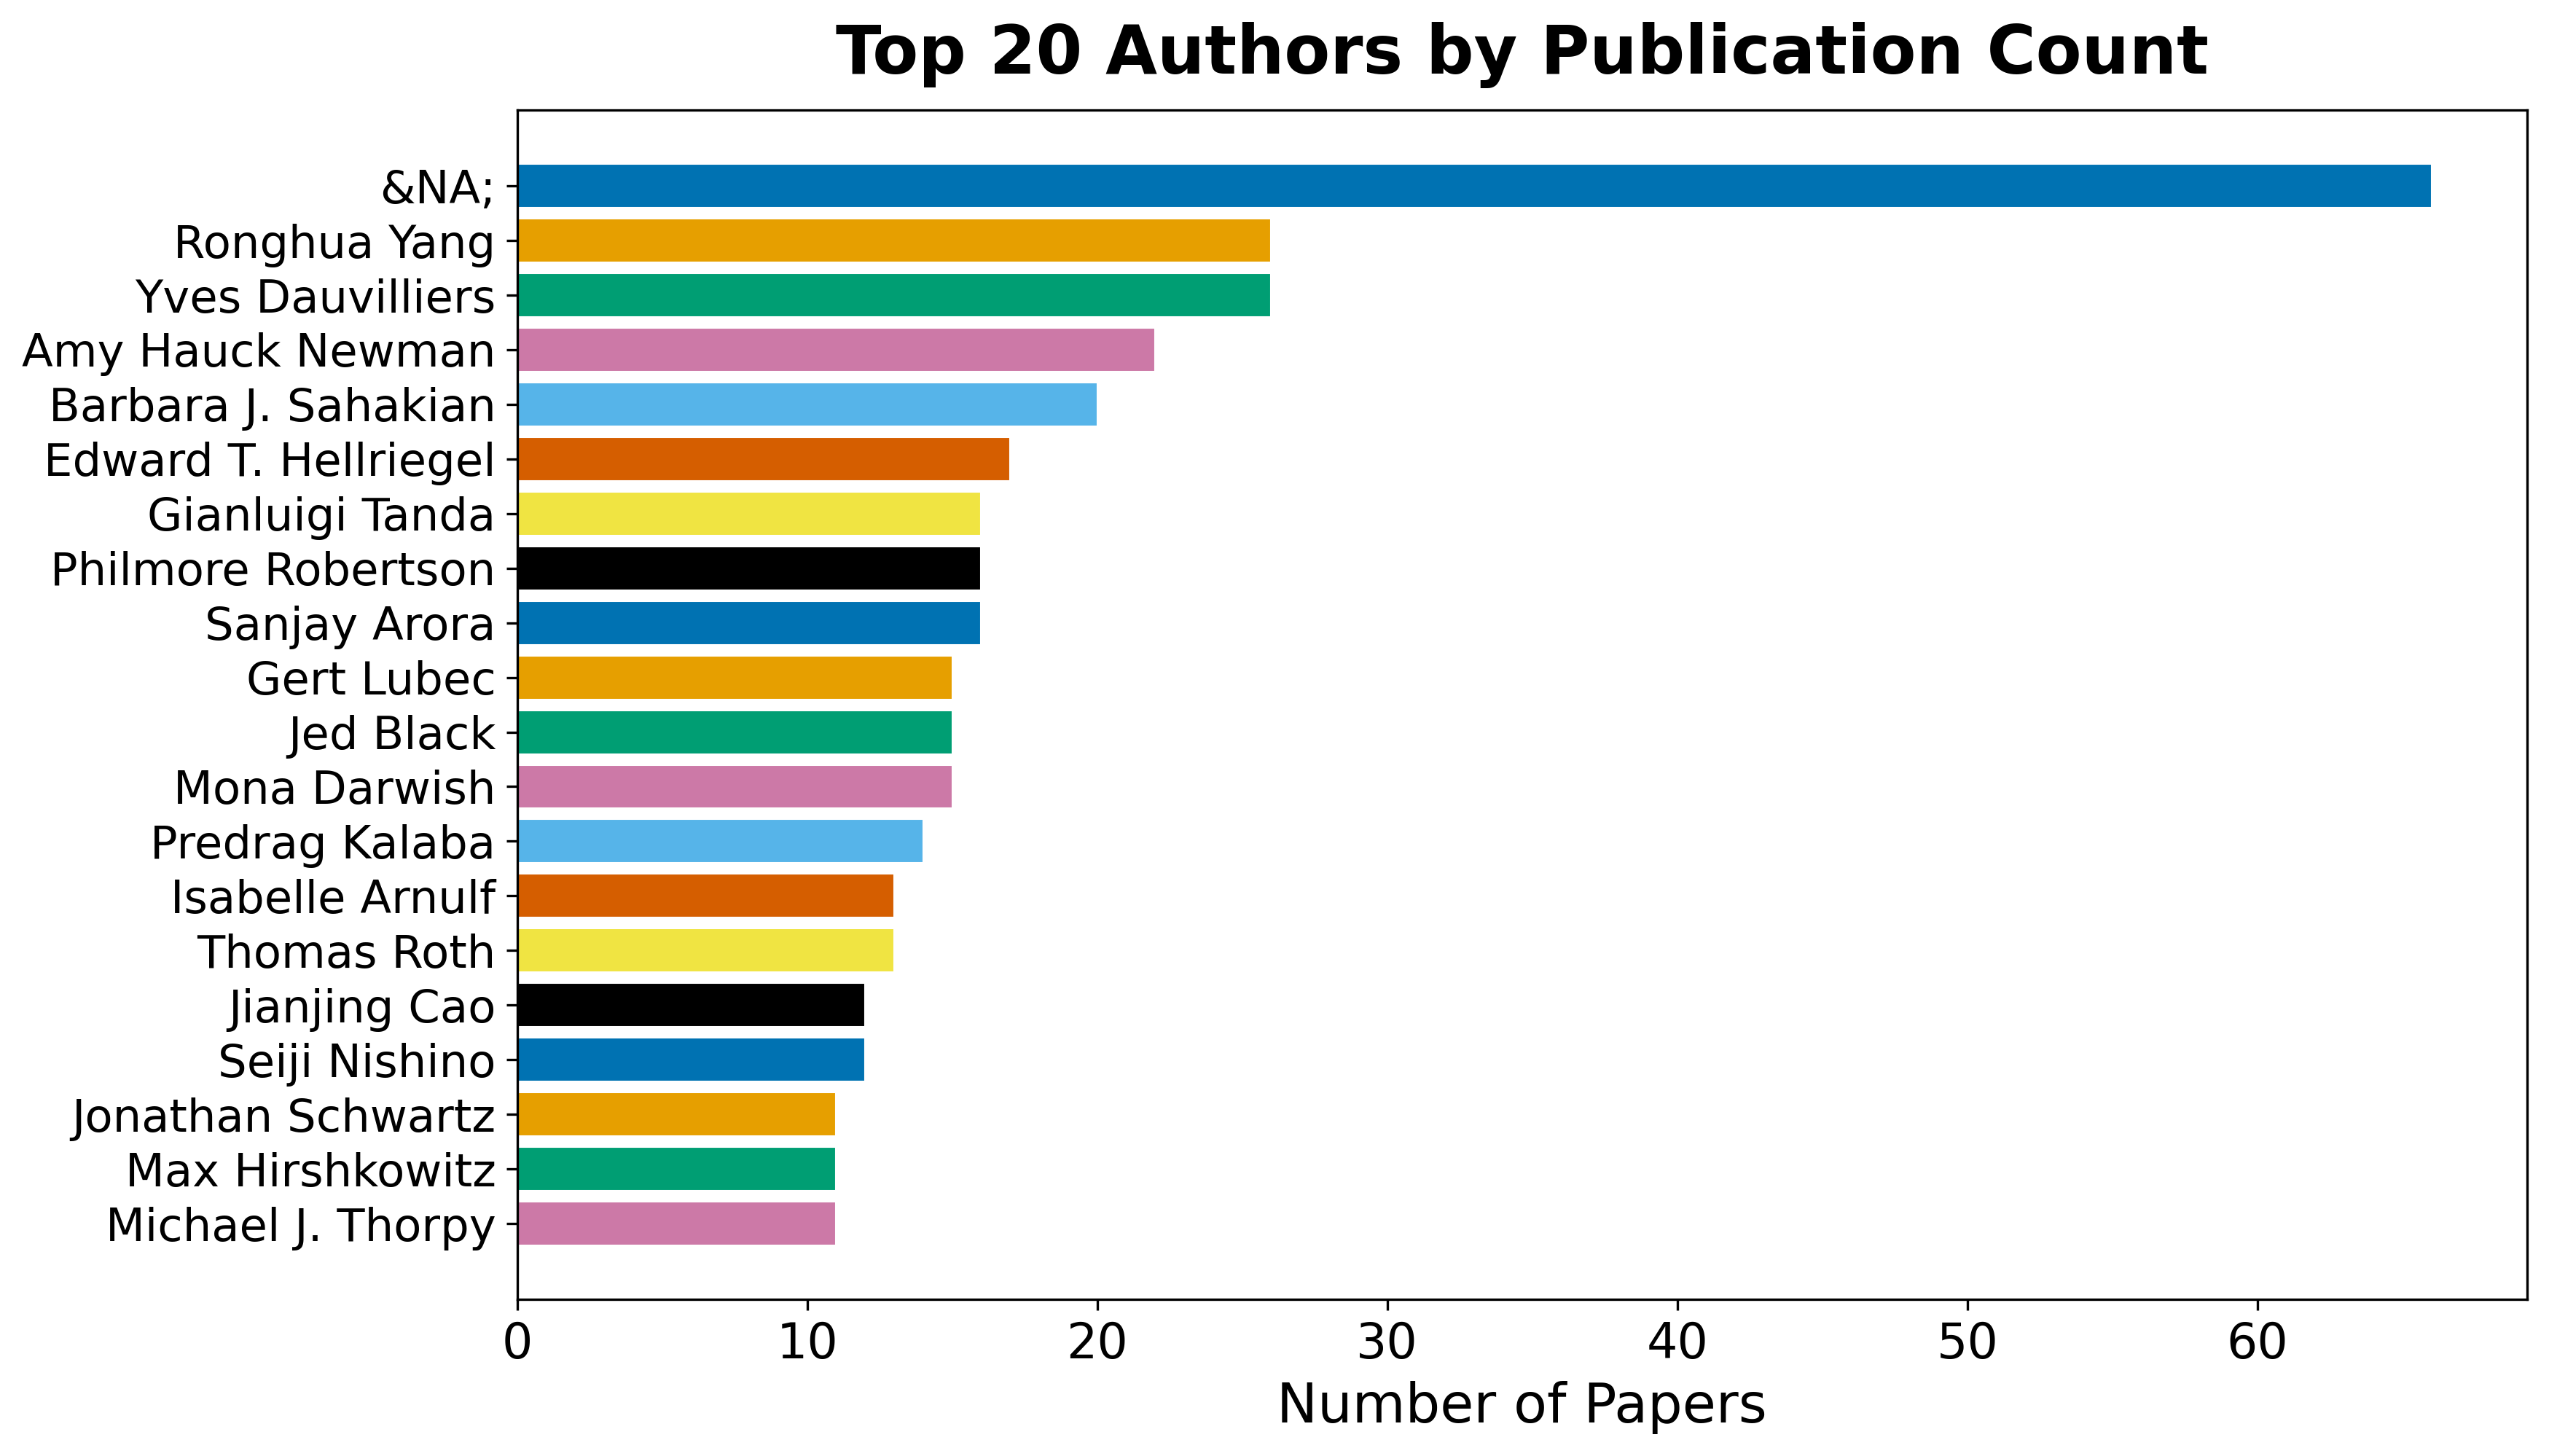
\includegraphics[keepaspectratio,alt={Author productivity for Modafinil. The horizontal bar chart shows the 20 authors with the most papers in the corpus, revealing the most prolific contributors to the modafinil literature.}]{../figures/author_productivity.png}}\{\{\#fig:author\_productivity\}\}
\end{frame}

\end{document}
